% Copyright 2013 Nicolai Hähnle <nhaehnle@gmail.com>
%
% This work is licensed under the Creative Commons Attribution-ShareAlike 3.0
% Unported License, see http://creativecommons.org/licenses/by-sa/3.0/
%
% Among other things, this means that yes, you may take e.g. illustrations from
% the book and use them in your own work. However, (a) you must give proper
% attribution by naming me as its original author and (b) you must make your
% derivative work available under the same or similar license terms.
%
% See the Creative Commons website for the exact licensing terms.

\chapter{Arbitrary Norms and Enumeration of Lattice Points}

We have seen how to find shortest and closest vectors in a lattice
with respect to the Euclidean norm in time $2^{O(d)} \cdot \poly(b)$,
where $b$ is the encoding size of the input.
What about the related problems with respect to an arbitrary norm $\|\cdot\|$?

In the decision variant of the closest vector problem,
we are given a lattice $\Lambda \subset \R^d$,
target vector $t \in \R^d$
and target distance $r > 0$,
and we have to decide whether there is a lattice point $x \in \Lambda$
with $\|x - t\| \leq r$.
This is a lattice programming problem:
decide whether the norm ball $B_{\|\cdot\|}(t,r)$ contains a lattice point.
We have seen that such problems can be solved in
$2^{O(d \log d)} \cdot \poly(b)$ arithmetic operations
and calls to an oracle describing $B_{\|\cdot\|}(t,r)$,
where $b$ is an upper bound on the encoding size of the problem,
including the logarithm of a bound on the size of $B_{\|\cdot\|}(t,r)$.
There is a gap between this running time and
the time we could previously achieve for the Euclidean norm.

We do not know how to adapt the techniques based on Voronoi cells
since Voronoi diagrams in other norms are rather complicated.
For one thing, Voronoi cells with respect to arbitrary norms are not even convex in general.

A different approach is needed.
Suppose we could somehow enumerate the lattice points in any convex body efficiently,
by an output-sensitive algorithm,
in time $(N+1)\cdot 2^{O(d)}$
where $N$ is the number of lattice points that are found.
Then a natural algorithm for solving the shortest vector problem is as follows:
Start with a lower bound $r = r_0$ on the $\|\cdot\|$-length of a shortest vector
and enumerate lattice points in the $\|\cdot\|$-ball of radius $r$ around the origin.
If a non-zero lattice point is found, output the shortest among them.
Otherwise, multiply $r$ by a constant factor and repeat.

Due to a volume argument,
the first $\|\cdot\|$-ball to contain \emph{any} non-zero lattice points
can only contain $2^{O(d)}$ of them.
Then the overall running time is still bounded by a single-exponential factor
times the logarithm of the quality of the initial estimate $r_0$.

In this chapter,
we will visit some theory on arbitrary norms,
develop a lattice point enumeration algorithm,
and use it to solve the shortest vector problem
and approximate the closest vector problem
with respect to arbitrary norms.

This approach is based on~\cite{DPV10}
and in fact works for \emph{semi-norms} and non-symmetric convex bodies.
However, we will restrict ourselves to the case of symmetric bodies
to simplify the presentation.


\section{Norms and Convex Bodies}

The unit ball
$B_{\|\cdot\|}(0,1)$
with respect to an arbitrary norm $\|\cdot\|$
is a compact convex set of positive volume.
Furthermore, it is \emph{symmetric}
in the sense that $B_{\|\cdot\|}(0,1) = -B_{\|\cdot\|}(0,1)$.

\begin{definition}
  Let $K$ be a symmetric, compact, convex set of positive volume.
  We define the norm associated to $K$ as
  \[
    \| x \|_K := \min\{ r \geq 0 ~:~ x \in r K \}
  \]
\end{definition}


\begin{lemma}
  $\|\cdot\|_K$ is a norm.
\end{lemma}
\begin{proof}
  Since $K$ has positive volume, is symmetric and convex,
  it contains a ball $B(0,\varepsilon)$ for some $\varepsilon > 0$.
  For any $x \neq 0$, this implies $x \in \frac{\|x\|_2}{\varepsilon} K$.
  So $\|x\|_K$ is well-defined for all $x \in \R^d$
  with $\|x\|_K = 0$ if and only if $x = 0$.

  In addition, we need to show $\|\lambda x\|_K = |\lambda| \cdot \|x\|_k$
  and the triangle inequality.
  By definition and using symmetry,
  \begin{align*}
    \|\lambda x\|_K
      &= \min\{ r \geq 0 ~:~ \lambda x \in r K \}
      = \min\{ r \geq 0 ~:~ x \in \frac{r}{|\lambda|} K \}
 \\ & = \min\{ |\lambda| r \geq 0 ~:~ x \in r K \}
      = |\lambda| \cdot \|x\|_K
  \end{align*}
  Let $x, y \in \R^d$.
  We have $x \in \|x\|_K \cdot K$ and $y \in \|y\|_K \cdot K$.
  Intuitively, the idea is that
  \[
    x + y \in \|x\|_K \cdot K + \|y\|_K \cdot K = (\|x\|_K + \|y\|_K) K
  \]
  and therefore $\|x+y\|_K \leq \|x\|_K + \|y\|_K$.
  The last equality of sets holds for general convex sets.
  We only need inclusion from left to right.
  Any $z \in \lambda K + \mu K$ can be written as $z = x + y$
  with $x \in \lambda K$ and $y \in \mu K$ by definition.
  \begin{align*}
    z = x + y = \lambda \cdot \underbrace{\frac{x}{\lambda}}_{\in K}
      + \mu \cdot \underbrace{\frac{y}{\mu}}_{\in K} \in (\lambda + \mu) K
  \end{align*}
  by convexity.
\end{proof}



\section{The polar of a convex body}

\begin{definition}
  Let $K \subset \R^d$ be a convex set.
  The \emph{polar} of $K$ is defined as
  \[
    K^\star := \{ y \in \R^d ~:~ y^Tx \leq 1 \,\forall x \in K \}
  \]
\end{definition}

The polar is sometimes also called the dual of a convex body.
Even though that terminology is also useful,
for example due to the connection to dual lattices that we will see,
we prefer the term polar so as not get confused with linear programming duality.
While the definition can be written down for arbitrary convex sets,
we will see that it is most meaningful for sets that contain $0$.

\begin{example}
  The cube $[-1,+1]^d$ is the polar of the cross polytope $\conv\{\pm e_j\}$ and vice versa.
  \begin{center}
    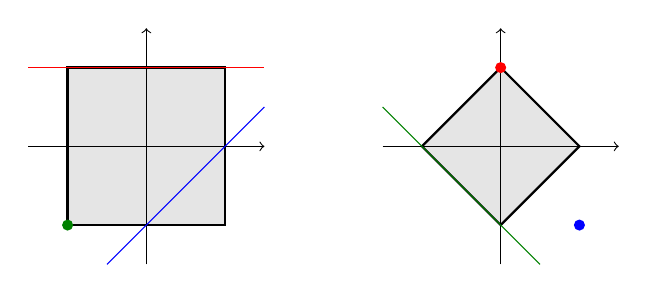
\begin{tikzpicture}
      \draw[thick,fill=black!10] (-1,-1) -- (1,-1) -- (1,1) -- (-1,1) -- cycle;
      \draw[->] (-1.5,0) -- (1.5,0);
      \draw[->] (0,-1.5) -- (0,1.5);

      \draw[thick,fill=black!10] (3.5,0) -- (4.5,-1) -- (5.5,0) -- (4.5,1) -- cycle;
      \draw[->] (3,0) -- (6,0);
      \draw[->] (4.5,-1.5) -- (4.5,1.5);

      \draw[red] (-1.5,1) -- (1.5,1);
      \fill[red] (4.5,1) circle[radius=2pt];

      \draw[blue] (-0.5,-1.5) -- (1.5,0.5);
      \fill[blue] (5.5,-1) circle[radius=2pt];

      \draw[green!50!black] (3,0.5) -- (5,-1.5);
      \fill[green!50!black] (-1,-1) circle[radius=2pt];
    \end{tikzpicture}
  \end{center}
  Valid inequalities of $K$ correspond to points of $K^\star$ and vice versa,
  as some examples in the drawing indicate.
\end{example}

\begin{lemma}
  Let $K \subseteq \R^d$ be a convex set.
  \begin{enumerate}
    \item $K^\star$ is a closed convex set that contains the origin.
    \item If $K$ is bounded, then $0 \in \operatorname{int} K^\star$.
    \item If $0 \in \operatorname{int} K$, then $K^\star$ is bounded.
    \item $K_1 \subseteq K_2$ implies $K_1^\star \supseteq K_2^\star$.
    \item $K \subseteq (K^\star)^\star$
    \item If $K$ is closed and contains the origin, then $(K^\star)^\star = K$.
  \end{enumerate}
\end{lemma}
\begin{proof}
  For the first point, observe that $K^\star$ can be written as the (infinite) intersection
  of closed half-spaces and $0 \in K^\star$ is obvious.

  For the second point, let $K \subseteq B(0, R)$
  and let $y \in B(0, 1/R)$.
  Then for all $x \in K$, one has
  \[
    y^T x \leq \|x\|_2 \|y\|_2 \leq 1
  \]
  Hence $B(0,1/R) \subseteq K^\star$

  For the third point, suppose $B(0,\varepsilon) \subseteq K$.
  Let $y \in K^\star$.
  Observe that $x := \varepsilon \frac{y}{\|y\|_2} \in K$,
  and so we have
  \[
    1 \geq y^Tx = \varepsilon \frac{y^Ty}{\|y\|_2} = \varepsilon \|y\|_2
  \]
  This implies $\|y\|_2 \leq 1/\varepsilon$, hence $K^\star$ is bounded.

  For the fourth point, observe that $y \in K_2^\star$
  satisfies $y^Tx \leq 1$ for all $x \in K_2$.
  In particular, it satisfies $y^Tx \leq 1$ for all $x \in K_1$,
  hence $y \in K_1^\star$.

  For the fifth point,
  let $x \in K$.
  We have $y^Tx \leq 1$ for all $y \in K^\star$ (by the definition of $K^\star$)
  and so (by the definition of $(K^\star)^\star$) we have $x \in (K^\star)^\star$.

  For the last point,
  it remains to be shown that $(K^\star)^\star \subseteq K$.
  Suppose, by way of contradiction,
  that there exists a point $z \in (K^\star)^\star$ with $z \not\in K$.
  Since $K$ is closed,
  there is a hyperplane that strictly separates $z$ from $K$.
  Formally, there exists a hyperplane with equation $a^Tx = b$
  with $a^Tx < b$ for all $x \in K$ and $a^Tz > b$.

  Since $0 \in K$, we have $b > 0$.
  By rescaling, we can ensure $b = 1$, which implies $a \in K^\star$.
  But since $a^Tz > b = 1$, this contradicts $z \in (K^\star)^\star$.
\end{proof}

\begin{lemma}
  Let $A \in \R^{d \times d}$ be an invertible matrix.
  Then $(A K)^\star = A^{-T} K^\star$.
\end{lemma}
\begin{proof}
  This follows from a simple chain of equivalences,
  the heart of which is the fact that $y^T(Ax) = (A^T y)^T x$.
\end{proof}

The polar of a convex body is related to its primal in the same way
that a dual lattice is related to its primal as per Corollary~\ref{corollary:transformed-dual-lattice}.
Indeed, when working in a lattice $\Lambda$ with respect to a norm $\|\cdot\|_K$,
we should work in its dual with respect to the norm $\|\cdot\|_{K^\star}$.
Let us extend the covering radius and the successive minima to general norms in the natural way,
where $K$ is a symmetric convex body of positive volume:
\begin{align*}
  \lambda_j(\Lambda, K) &:= \min\{ r > 0 ~:~ \dim( \Lambda \cap B_{\|\cdot\|_K}(0,r) ) \geq j \} \\
  \mu(\Lambda, K) &:= \max_{p \in \R^d} d_{\|\cdot\|_K}(p, \Lambda)
\end{align*}
We can immediately extend some of the statements from Chapter~\ref{chapter:dual-lattices}.
\begin{lemma}
  The lattice width of $K$ is related to the length of a shortest vector by
  $w(K,\Lambda) = 2\lambda_1(\Lambda^\star, K^\star)$.
\end{lemma}
\begin{proof}
  Let $y \in \Lambda^\star$.
  \begin{align*}
    w_y(K) = \max_{x \in K} y^Tx - \min_{x \in K} y^Tx = 2 \max_{x \in K} y^Tx
  \end{align*}
  by symmetry.
  Read differently, we have
  \[
    y^Tx \leq \frac{w_y(K)}{2}
  \]
  for all $x \in K$, which implies $y \in \frac{w_y(K)}{2} K^\star$.
  On the other hand, there is an $x \in K$ that satisfies the inequality with equality,
  and hence $w_y(K) / 2$ is the smallest possible factor by which $K^\star$ must be scaled to contain $y$,
  i.e. $\|y\|_{K^\star} = w_y(K) / 2$.
  \[
    w(K,\Lambda) = \min_{y\in K^\star\setminus 0} w_y(K) = \min_{y\in K^\star\setminus 0} 2 \|y\|_{K^\star}
      = 2 \lambda_1(\Lambda^\star, K^\star) \qedhere
  \]
\end{proof}

\begin{lemma}[Flatness Lemma]
  Suppose one has $\lambda_1^\star(\Lambda^\star, K^\star) \cdot \mu(\Lambda, K) \leq c_d$
  for all lattices $\Lambda \subset \R^d$ and symmetric convex bodies $K \subseteq \R^d$.
  Then $w(K,\Lambda) \geq 2c_d$ implies that $p + K$ contains a lattice point for every $p \in \R^d$.
\end{lemma}
\begin{proof}
  By the previous Lemma, $2c_d \leq w(K,\Lambda) = 2 \lambda_1^\star(\Lambda^\star, K^\star)$.
  This implies $\mu(\Lambda, K) \leq 1$,
  which by definition means that for every $p \in \R^d$,
  there is an $x \in \Lambda$ with $\|p - x\|_K \leq 1$.
  But then $x \in p + K$.
\end{proof}







\section{Enumerating lattice points in an ellipsoid}



\section{Some examples on enumeration}

Now that we can enumerate lattice points in an ellipsoid,
a natural idea for enumerating points in a more general body $K$
is to take an ellipsoid $E$ of smallest volume enclosing $K$.
However, this approach cannot lead to an efficient algorithm.

Consider the cube
\[
  P := [-1, +1]^d,
\]
whose smallest enclosing ellipsoid is the $\ell_2$ ball $B = B(0,\sqrt{d})$.
Let us place a cube




\section*{Exercises}

\begin{enumerate}
  \item Show: $K^\star = K$ if and only if $K$ is the closed Euclidean unit ball.
\end{enumerate}
